\documentclass[aps,prb,
superscriptaddress,
%,twocolumn
,floatfix,footinbib,longbibliography,
preprint
]{revtex4-2}
%\documentclass[aps,preprint,floatfix,footinbib,longbibliography]{revtex4-1}
\usepackage{epsfig}
\usepackage{graphicx}% Include figure files
\usepackage{dcolumn}% Align table columns on decimal point
\usepackage{bm}% bold math
\usepackage{mathrsfs}
\usepackage{amsmath}
\usepackage{bbold}
\usepackage{color,xcolor}
\usepackage{epstopdf}
\usepackage{subfigure}
\usepackage{footmisc}
%\newcommand{\equt}[1]{\stackrel{#1}{=}}
%\usepackage[backend=bibtex,sorting=none,style=trad-abbrv,citestyle=numeric]{biblatex}

%\usepackage[sorting=none]{biblatex}
%\usepackage{hyperref}
%\usepackage[titletoc]{appendix}
% avoids incorrect hyphenation, added Nov/08 by SSR
\hyphenation{ALPGEN}
\hyphenation{EVTGEN}
\hyphenation{PYTHIA}

\usepackage[colorlinks=true,pdfborder=001,linkcolor=blue,anchorcolor=blue,citecolor=blue,urlcolor=blue]{hyperref}

\newcommand{\revision}[1]{{\color{blue}{#1}}}
\newcommand{\JT}[1]{{\color{red}{#1}}}
\begin{document}

%\preprint{APS/123-QED}

\title{Supplemental Material for  ``Effective control of photon statistics from electroluminescence by Fano-like interference effect"}%
\author{Lei-Lei Nian}
\affiliation{School of Physics and Wuhan National High Magnetic Field Center, Huazhong University of Science and Technology, Wuhan 430074, P. R. China}
\author{Tao Wang}
\affiliation{School of Physics and Wuhan National High Magnetic Field Center, Huazhong University of Science and Technology, Wuhan 430074, P. R. China}
\author{Zu-Quan Zhang}
\affiliation{Department of Physics, National University of Singapore, Singapore 117551, Republic of Singapore}
\author{Jian-Sheng Wang}
%\email{phywjs@nus.edu.sg}
\affiliation{Department of Physics, National University of Singapore, Singapore 117551, Republic of Singapore}
\author{Jing-Tao L\"{u}}
\email{jtlu@hust.edu.cn}
\affiliation{School of Physics and Wuhan National High Magnetic Field Center, Huazhong University of Science and Technology, Wuhan 430074, P. R. China}

\date{\today}% It is always \today, today,
             %  but any date may be explicitly specified


%\pacs{73.63.kv, 73.23.-b, 71.38.-k}% PACS, the Physics and Astronomy
                             % Classification Scheme.
%\keywords{Suggested keywords}%Use showkeys class option if keyword
                              %display desired
\maketitle
%\section{Introduction}
\revision{
\section{Hamiltonian of the environment and its coupling with system}
Hamiltonian of the environment and its coupling with system are $\mathcal{H}_{en}$ and $\mathcal{H}_{en-s}$, respectively. Here $\mathcal{H}_{en}$ contains electrodes $\mathcal{H}_{elec}$ and photon bath $\mathcal{H}_{ph}$
\begin{equation}
\begin{split}
&\mathcal{H}_{en}=\mathcal{H}_{elec}+\mathcal{H}_{ph},\\  
&\mathcal{H}_{elec}=\sum_{k_{\alpha\nu};\alpha\in L,R;\nu\in p,m}\varepsilon_{k_{\alpha1}}c_{k_{\alpha \nu}}^{\dagger}c_{k_{\alpha \nu}},\\
&\mathcal{H}_{ph}=\sum_{q}\hbar\omega_{q}(\frac{1}{2}+a_{q}^{\dagger}a_{q}),\\
\end{split}
\end{equation}
where the subscript $\nu$ labels two electrical subsystems that can be used to excite the molecules p and m, $c_{k_{\alpha \nu}}^{\dagger}~(c_{k_{\alpha \nu}})$ is the creation (annihilation) operator of an
electron with energy $\varepsilon_{k_{\alpha \nu}}$ in the electrode $\alpha$ of subsystem $\nu$. In $\mathcal{H}_{ph}$, $a_{q}^{\dagger}~(a_{q})$ is the creation (annihilation) operator of a photon with angular frequency $\omega_{q}$ in the photon bath.

The environment-system interaction can be expressed as
\begin{equation}
\begin{split}
\mathcal{H}_{en-s}=\mathcal{H}_{mole-elec}+\mathcal{H}_{c-ph}+\mathcal{H}_{mole-ph},
\end{split}
\end{equation}
where $\mathcal{H}_{mole-elec}=\mathcal{H}_{p-elec}+\mathcal{H}_{m-elec}$ describes the the coupling between the molecules and the electrodes. For molecule $p$, we have
\begin{equation}
\begin{split}
\mathcal{H}_{p-elec}&=\sum_{k_{Lp}}(t_{Lp,e}c_{k_{Lp}}^{\dagger}d_{e}+t_{Lp,e}^{\ast}d_{e}^{\dagger}c_{k_{Lp}})+\sum_{k_{Rp}}(t_{Rp,g}c_{k_{Rp}}^{\dagger}d_{g}+t_{Rp,g}^{\ast}d_{g}^{\dagger}c_{k_{Rp}}),
\end{split}
\label{molecule-electrode}
\end{equation}
Similar expressions can be written for $\mathcal{H}_{m-elec}$.
%
$\mathcal{H}_{c-ph}$ describes the coupling between cavity mode and photon bath
\begin{equation}
\mathcal{H}_{c-ph}=\sum_{q}(t_{qc}a_{q}^{\dagger}a_{c}+t_{qc}^{\ast}a_{c}^{\dagger}a_{q}),
\end{equation}
where $t_{qc}$ is the coupling constant. 

$\mathcal{H}_{mole-ph}$ describes the coupling between molecule and photon bath
\begin{equation}
\mathcal{H}_{mole-ph}=\sum_{q;\nu=p,m}(t_{qmo}a_{q}^{\dagger}\sigma_{\nu}+t_{qmo}^{\ast}\sigma_{\nu}^{\dagger}a_{q}),
\end{equation}
where $t_{qmo}$ characterizes the coupling strength.
%
Here we assume that the photon bath is in thermal equilibrium, then the photons in the bath obey Bose-Einstein distribution $n_{B}(\omega)=(e^{\hbar\omega/k_{B}T}-1)^{-1}$.
The coupling between the cavity mode and the bath can be expressed as $\gamma_{c}=2\pi\sum_{q}\left| t_{qc }\right|^{2}\delta(\omega-\omega_{c})$.
Similarly, $\gamma_{d\nu}=2\pi\sum_{q}\left| t_{qmo }\right|^{2}\delta(\omega-\omega_{\nu})$, with $\hbar\omega_\nu$  the molecular level separation.

The excitation (b, d) and de-excitation (a, c) of molecular exciton by the electrical pumping can be expressed in the following processes 
\begin{equation}
\begin{split}
&\underbrace{\sum_{k_{Lp}}\sum_{k_{Rp}}t_{Lp,e}t_{Rp,g}^{\ast}c_{k_{Lp}}^{\dagger}c_{k_{Rp}}\sigma_p}_{(a)}+\underbrace{\sum_{k_{Lp}}\sum_{k_{Rp}}t_{Lp,e}^{\ast}t_{Rp,g}c_{k_{Rp}}^{\dagger}c_{k_{Lp}}\sigma_p^\dagger}_{(b)}\\
&+\underbrace{\sum_{k_{Lm}}\sum_{k_{Rm}}t_{Lm,l}t_{Rm,h}^{\ast}c_{k_{Lm}}^{\dagger}c_{k_{Rm}}\sigma_m}_{(c)}+\underbrace{\sum_{k_{Lm}}\sum_{k_{Rm}}t_{Lm,l}^{\ast}t_{Rm,h}c_{k_{Rm}}^{\dagger}c_{k_{Lm}}\sigma_m^\dagger}_{(d)},
\end{split}
\label{exciton-electrode}
\end{equation}
where $\sigma_p = d_{g}^{\dagger}d_{e}$ ($\sigma_m=d_{h}^{\dagger}d_{l}$) and $\sigma_p^\dagger=d_{e}^{\dagger}d_{g}$ ($\sigma_m^\dagger=d_{l}^{\dagger}d_{h}$) are the annihilation and creation operators of molecular exciton p (m).   
With this, the rates $\Gamma_{\nu}^{+}$ and $\Gamma_{\nu}^{-}$ in Eq.~6 of the main text can be obtained. For example, we have for molecule $p$
\begin{equation}
\begin{split}
&\Gamma_{p}^{+}=E_{p}f_{p}^{e},
\quad \Gamma_{p}^{-}=E_{p}(1-f_{p}^{e}),
\end{split}
\end{equation}
where $E_{p}=\sum_{k_{Lp},k_{Rp}}|t_{Lp,e}|^2 |t_{Rp,g}|^2\delta(\varepsilon_{k_{Lp}}-\varepsilon_e)\delta(\varepsilon_{k_{Rp}}-\varepsilon_g)$. We take the tunnel matrix elements to be constant.
%We have assumed that $eV_{j}>\hbar\omega_{j}$, then $f_{j}^{e}=1$ at low-temperature limit. In this case, we have $\Gamma_{p}^{+}=E_{p}$, $\Gamma_{m}^{+}=E_{m}$, $\Gamma_{p}^{-}=0$, and $\Gamma_{m}^{-}=0$.
The joint occupation can be evaluated as
\begin{equation}
\begin{split}
f_{p}^{e}&=
\langle c_{k_{Lp}}^{\dagger}c_{k_{Lp}}\rangle \langle c_{k_{Rp}} c_{k_{Rp}}^{\dagger}\rangle\\
&=n_{F}^{Lp}(\varepsilon_{e})[1-n^{Rp}_{F}(\varepsilon_{g})]\\
&=-n_{B}(\hbar\omega_{p}-eV_{p})[n^{Lp}_{F}(\varepsilon_{e})-n^{Rp}_{F}(\varepsilon_{g})],\\
\end{split}
\end{equation}
where $n_{F}^{\alpha p}(\varepsilon)=(e^{(\varepsilon-\mu_{\alpha  p})/k_{B}T}+1)^{-1}$ is the  Fermi-Dirac distribution with the chemical potential $\mu_{\alpha p}$ and the temperature $T$,  
$eV_{p}=\mu_{Lp}-\mu_{Rp}$ is bias voltage between electrodes $Lp$ and $Rp$. We consider the case where level $e$ couples only to the left and $g$ only to the right electrode. When $\mu_{Lp} \gg \varepsilon_e > \varepsilon_g \gg \mu_{Rp}$, we have $f_p^e = 1$, thus $\Gamma_p^+=E_{p}$ and $\Gamma_p^-=0$. We can consider pumping of molecule $m$ in the same way.

}



\section{Matrix elements of the density operator}
\label{matrix}

We can define the molecule-cavity reduced density operator
\begin{equation}
\rho_{m,n}^{ij,i^{\prime}j^{\prime}}:=\langle m,i,i^{\prime}|\rho|j^{\prime},j,n \rangle,
\end{equation}
where $i,j=g,e$ and $i^{\prime},j^{\prime}=h,l$. $m$ and $n$ represent the photon Fock states in the cavity. The Coulomb interaction
between two levels in each molecule is assumed very strong, such that only one additional electron can
 occupy the molecule at a time. In this case, for given $m$ and $n$, 16 linear equations for the matrix elements can be obtained. Here, their detailed expressions are not shown.
 %as shown in Fig.~\ref{figure:master-p},

 %
 \iffalse
 
\begin{equation}
\begin{split}
\frac{d}{dt}\rho_{m,n}^{hh,gg}&=-i\hbar\omega_{c}(m-n)\rho_{m,n}^{hh,gg}+\gamma_{dm}\rho_{m,n}^{ll,gg}
-E_{m}\rho_{m,n}^{hh,gg}
+\gamma_{dp}\rho_{m,n}^{hh,ee}-E_{p}\rho_{m,n}^{hh,gg}\\
&-im_{ep}(\sqrt{m}\rho_{m-1,n}^{lh,gg}-\sqrt{n}\rho_{m,n-1}^{hl,gg})
-im_{p}(\sqrt{m}\rho_{m-1,n}^{hh,eg}-\sqrt{n}\rho_{m,n-1}^{hh,ge})\\
&+\frac{\gamma_{c}}{2}[2\sqrt{m+1}\sqrt{n+1}\rho_{m+1,n+1}^{hh,gg}-(m+n)\rho_{m,n}^{hh,gg}].\\
\end{split}
\label{hh,gg}
\end{equation}
%
\begin{equation}
\begin{split}
\frac{d}{dt}\rho_{m,n}^{hh,ee}&=-i\hbar\omega_{c}(m-n)\rho_{m,n}^{hh,ee}+\gamma_{dm}\rho_{m,n}^{ll,ee}
-E_{m}\rho_{m,n}^{hh,ee}-\gamma_{dp}\rho_{m,n}^{hh,ee}+E_{p}\rho_{m,n}^{hh,gg}\\
&-im_{ep}(\sqrt{m}\rho_{m-1,n}^{lh,ee}-\sqrt{n}\rho_{m,n-1}^{hl,ee})
-im_{p}(\sqrt{m+1}\rho_{m+1,n}^{hh,ge}-\sqrt{n+1}\rho_{m,n+1}^{hh,eg})\\
&+\frac{\gamma_{c}}{2}[2\sqrt{m+1}\sqrt{n+1}\rho_{m+1,n+1}^{hh,ee}-(m+n)\rho_{m,n}^{hh,ee}].\\
\end{split}
\label{hh,ee}
\end{equation}
%
\begin{equation}
\begin{split}
\frac{d}{dt}\rho_{m,n-1}^{hh,ge}&=-i\hbar\omega_{c}(m-n+1)\rho_{m,n-1}^{hh,ge}
-i(\varepsilon_{g}-\varepsilon_{e})\rho_{m,n-1}^{hh,ge}\\
&+\gamma_{dm}\rho_{m,n-1}^{ll,ge}
-E_{m}\rho_{m,n-1}^{hh,ge}-(\frac{\gamma_{dp}}{2}+\frac{E_{p}}{2})\rho_{m,n-1}^{hh,ge}\\
&-im_{ep}(\sqrt{m}\rho_{m-1,n-1}^{lh,ge}-\sqrt{n-1}\rho_{m,n-2}^{hl,ge})
-im_{p}(\sqrt{m}\rho_{m-1,n-1}^{hh,ee}-\sqrt{n}\rho_{m,n}^{hh,gg})\\
&+\frac{\gamma_{c}}{2}[2\sqrt{m+1}\sqrt{n}\rho_{m+1,n}^{hh,ge}-(m+n-1)\rho_{m,n-1}^{hh,ge}].\\
\end{split}
\label{hh,ge}
\end{equation}
%
%\begin{equation}
%\begin{split}
%\frac{d}{dt}\rho_{m-1,n}^{hh,eg}&=-i\hbar\omega_{c}(m-n-1)\rho_{m-1,n}^{hh,eg}
%-i(\varepsilon_{e}-\varepsilon_{g})\rho_{m-1,n}^{hh,eg}\\
%&+\gamma_{dm}\rho_{m-1,n}^{ll,eg}
%-E_{m}\rho_{m-1,n}^{hh,eg}-(\frac{\gamma_{dp}}{2}+\frac{E_{p}}{2})\rho_{m-1,n}^{hh,eg}\\
%&-im_{ep}(\sqrt{m-1}\rho_{m-2,n}^{lh,eg}-\sqrt{n}\rho_{m-1,n-1}^{hl,eg})
%-im_{p}(\sqrt{m}\rho_{m,n}^{hh,gg}-\sqrt{n}\rho_{m-1,n-1}^{hh,ee})\\
%&+\frac{\gamma_{c}}{2}[2\sqrt{m}\sqrt{n+1}\rho_{m,n+1}^{hh,eg}-(m+n-1)\rho_{m-1,n}^{hh,eg}].\\
%\end{split}
%\end{equation}
%
\begin{equation}
\begin{split}
\frac{d}{dt}\rho_{m,n}^{ll,gg}&=-i\hbar\omega_{c}(m-n)\rho_{m,n}^{ll,gg}-\gamma_{dm}\rho_{m,n}^{ll,gg}
+E_{m}\rho_{m,n}^{hh,gg}+\gamma_{dp}\rho_{m,n}^{ll,ee}-E_{p}\rho_{m,n}^{ll,gg}\\
&-im_{ep}(\sqrt{m+1}\rho_{m+1,n}^{hl,gg}-\sqrt{n+1}\rho_{m,n+1}^{lh,gg})
-im_{p}(\sqrt{m}\rho_{m-1,n}^{ll,eg}-\sqrt{n}\rho_{m,n-1}^{ll,ge})\\
&+\frac{\gamma_{c}}{2}[2\sqrt{m+1}\sqrt{n+1}\rho_{m+1,n+1}^{ll,gg}-(m+n)\rho_{m,n}^{ll,gg}].\\
\end{split}
\label{ll,gg}
\end{equation}
%
\begin{equation}
\begin{split}
\frac{d}{dt}\rho_{m,n}^{ll,ee}&=-i\hbar\omega_{c}(m-n)\rho_{m,n}^{ll,ee}-\gamma_{dm}\rho_{m,n}^{ll,ee}
+E_{m}\rho_{m,n}^{hh,ee}-\gamma_{dp}\rho_{m,n}^{ll,ee}+E_{p}\rho_{m,n}^{ll,gg}\\
&-im_{ep}(\sqrt{m+1}\rho_{m+1,n}^{hl,ee}-\sqrt{n+1}\rho_{m,n+1}^{lh,ee})
-im_{p}(\sqrt{m+1}\rho_{m+1,n}^{ll,ge}-\sqrt{n+1}\rho_{m,n+1}^{ll,eg})\\
&+\frac{\gamma_{c}}{2}[2\sqrt{m+1}\sqrt{n+1}\rho_{m+1,n+1}^{ll,ee}-(m+n)\rho_{m,n}^{ll,ee}].\\
\end{split}
\label{ll,ee}
\end{equation}
%
\begin{equation}
\begin{split}
\frac{d}{dt}\rho_{m,n-1}^{ll,ge}&=-i\hbar\omega_{c}(m-n+1)\rho_{m,n-1}^{ll,ge}
-i(\varepsilon_{g}-\varepsilon_{e})\rho_{m,n-1}^{ll,ge}\\
&-\gamma_{dm}\rho_{m,n-1}^{ll,ge}+E_{m}\rho_{m,n-1}^{hh,ge}
-(\frac{\gamma_{dp}}{2}+\frac{{E_{p}}}{2})\rho_{m,n-1}^{ll,ge}\\
&-im_{ep}(\sqrt{m+1}\rho_{m+1,n-1}^{hl,ge}-\sqrt{n}\rho_{m,n}^{lh,ge})
-im_{p}(\sqrt{m}\rho_{m-1,n-1}^{ll,ee}-\sqrt{n}\rho_{m,n}^{ll,gg})\\
&+\frac{\gamma_{c}}{2}[2\sqrt{m+1}\sqrt{n}\rho_{m+1,n}^{ll,ge}-(m+n-1)\rho_{m,n-1}^{ll,ge}].\\
\end{split}
\label{ll,ge}
\end{equation}
%
%\begin{equation}
%\begin{split}
%\frac{d}{dt}\rho_{m-1,n}^{ll,eg}&=-i\hbar\omega_{c}(m-1-n)\rho_{m-1,n}^{ll,eg}
%-i(\varepsilon_{e}-\varepsilon_{g})\rho_{m-1,n}^{ll,eg}\\
%&-\gamma_{dm}\rho_{m-1,n}^{ll,eg}+E_{m}\rho_{m-1,n}^{hh,eg}
%-(\frac{\gamma_{dp}}{2}+\frac{{E_{p}}}{2})\rho_{m-1,n}^{ll,eg}\\
%&-im_{ep}(\sqrt{m}\rho_{m,n}^{hl,eg}-\sqrt{n+1}\rho_{m-1,n+1}^{lh,eg})
%-im_{p}(\sqrt{m}\rho_{m,n}^{ll,gg}-\sqrt{n}\rho_{m-1,n-1}^{ll,ee})\\
%&+\frac{\gamma_{c}}{2}[2\sqrt{m}\sqrt{n+1}\rho_{m,n+1}^{ll,eg}-(m+n-1)\rho_{m-1,n}^{ll,eg}].\\
%\end{split}
%\end{equation}
%
\begin{equation}
\begin{split}
\frac{d}{dt}\rho_{m,n-1}^{hl,gg}&=-i\hbar\omega_{c}(m-n+1)\rho_{m,n-1}^{hl,gg}
-i(\varepsilon_{h}-\varepsilon_{l})\rho_{m,n-1}^{hl,gg}\\
&-(\frac{\gamma_{dm}}{2}+\frac{E_{m}}{2})\rho_{m,n-1}^{hl,gg}
+\gamma_{dp}\rho_{m,n-1}^{hl,ee}-E_{p}\rho_{m,n-1}^{hl,gg}\\
&-im_{ep}(\sqrt{m}\rho_{m-1,n-1}^{ll,gg}-\sqrt{n}\rho_{m,n}^{hh,gg})
-im_{p}(\sqrt{m}\rho_{m-1,n-1}^{hl,eg}-\sqrt{n-1}\rho_{m,n-2}^{hl,ge})\\
&+\frac{\gamma_{c}}{2}[2\sqrt{m+1}\sqrt{n}\rho_{m+1,n}^{hl,gg}-(m+n-1)\rho_{m,n-1}^{hl,gg}].\\
\end{split}
\label{hl,gg}
\end{equation}
%
\begin{equation}
\begin{split}
\frac{d}{dt}\rho_{m,n-1}^{hl,ee}&=-i\hbar\omega_{c}(m-n+1)\rho_{m,n-1}^{hl,ee}
-i(\varepsilon_{h}-\varepsilon_{l})\rho_{m,n-1}^{hl,ee}\\
&-(\frac{\gamma_{dm}}{2}+\frac{E_{m}}{2})\rho_{m,n-1}^{hl,ee}
-\gamma_{dp}\rho_{m,n-1}^{hl,ee}+E_{p}\rho_{m,n-1}^{hl,gg}\\
&-im_{ep}(\sqrt{m}\rho_{m-1,n-1}^{ll,ee}-\sqrt{n}\rho_{m,n}^{hh,ee})
-im_{p}(\sqrt{m+1}\rho_{m+1,n-1}^{hl,ge}-\sqrt{n}\rho_{m,n}^{hl,eg})\\
&+\frac{\gamma_{c}}{2}[2\sqrt{m+1}\sqrt{n}\rho_{m+1,n}^{hl,ee}-(m+n-1)\rho_{m,n-1}^{hl,ee}].\\
\end{split}
\label{hl,ee}
\end{equation}
%
\begin{equation}
\begin{split}
\frac{d}{dt}\rho_{m,n-2}^{hl,ge}&=-i\hbar\omega_{c}(m-n+2)\rho_{m,n-2}^{hl,ge}
-i(\varepsilon_{h}-\varepsilon_{l})\rho_{m,n-2}^{hl,ge}-i(\varepsilon_{g}-\varepsilon_{e})\rho_{m,n-2}^{hl,ge}\\
&-(\frac{\gamma_{dm}}{2}+\frac{E_{m}}{2})\rho_{m,n-2}^{hl,ge}
-(\frac{\gamma_{dp}}{2}+\frac{E_{p}}{2})\rho_{m,n-2}^{hl,ge}\\
&-im_{ep}(\sqrt{m}\rho_{m-1,n-2}^{ll,ge}-\sqrt{n-1}\rho_{m,n-1}^{hh,ge})
-im_{p}(\sqrt{m}\rho_{m-1,n-2}^{hl,ee}-\sqrt{n-1}\rho_{m,n-1}^{hl,gg})\\
&+\frac{\gamma_{c}}{2}[2\sqrt{m+1}\sqrt{n-1}\rho_{m+1,n-1}^{hl,ge}-(m+n-2)\rho_{m,n-2}^{hl,ge}].\\
\end{split}
\label{hl,ge}
\end{equation}
%
\begin{equation}
\begin{split}
\frac{d}{dt}\rho_{m,n}^{hl,eg}&=-i\hbar\omega_{c}(m-n)\rho_{m,n}^{hl,eg}-i(\varepsilon_{h}-\varepsilon_{l})\rho_{m,n}^{hl,eg}
-i(\varepsilon_{e}-\varepsilon_{g})\rho_{m,n}^{hl,eg}\\
&-(\frac{\gamma_{dm}}{2}+\frac{E_{m}}{2})\rho_{m,n}^{hl,eg}
-(\frac{\gamma_{dp}}{2}+\frac{E_{p}}{2})\rho_{m,n}^{hl,eg}\\
&-im_{ep}(\sqrt{m}\rho_{m-1,n}^{ll,eg}-\sqrt{n+1}\rho_{m,n+1}^{hh,eg})
-im_{p}(\sqrt{m+1}\rho_{m+1,n}^{hl,gg}-\sqrt{n}\rho_{m,n-1}^{hl,ee})\\
&+\frac{\gamma_{c}}{2}[2\sqrt{m+1}\sqrt{n+1}\rho_{m+1,n+1}^{hl,eg}-(m+n)\rho_{m,n}^{hl,eg}].\\
\end{split}
\label{hl,eg}
\end{equation}
%
%\begin{equation}
%\begin{split}
%\frac{d}{dt}\rho_{m-1,n}^{lh,gg}&=-i\hbar\omega_{c}(m-1-n)\rho_{m-1,n}^{lh,gg}
%-i(\varepsilon_{l}-\varepsilon_{h})\rho_{m-1,n}^{lh,gg}\\
%&-(\frac{\gamma_{dm}}{2}+\frac{E_{m}}{2})\rho_{m-1,n}^{lh,gg}+
%\gamma_{dp}\rho_{m-1,n}^{lh,ee}-E_{p}\rho_{m-1,n}^{lh,gg}\\
%&-im_{ep}(\sqrt{m}\rho_{m,n}^{hh,gg}-\sqrt{n}\rho_{m-1,n-1}^{ll,gg})
%-im_{p}(\sqrt{m-1}\rho_{m-2,n}^{lh,eg}-\sqrt{n}\rho_{m-1,n-1}^{lh,ge})\\
%&+\frac{\gamma_{c}}{2}[2\sqrt{m}\sqrt{n+1}\rho_{m,n+1}^{lh,gg}-(m+n-1)\rho_{m-1,n}^{lh,gg}].\\
%\end{split}
%\end{equation}
%
%\begin{equation}
%\begin{split}
%\frac{d}{dt}\rho_{m-1,n}^{lh,ee}&=-i\hbar\omega_{c}(m-1-n)\rho_{m-1,n}^{lh,ee}
%-i(\varepsilon_{l}-\varepsilon_{h})\rho_{m-1,n}^{lh,ee}\\
%&-(\frac{\gamma_{dm}}{2}+\frac{E_{m}}{2})\rho_{m-1,n}^{lh,ee}
%-\gamma_{dp}\rho_{m-1,n}^{lh,ee}+E_{p}\rho_{m-1,n}^{lh,gg}\\
%&-im_{ep}(\sqrt{m}\rho_{m,n}^{hh,ee}-\sqrt{n}\rho_{m-1,n-1}^{ll,ee})
%-im_{p}(\sqrt{m}\rho_{m,n}^{lh,ge}-\sqrt{n+1}\rho_{m-1,n+1}^{lh,eg})\\
%&+\frac{\gamma_{c}}{2}[2\sqrt{m}\sqrt{n+1}\rho_{m,n+1}^{lh,ee}-(m+n-1)\rho_{m-1,n}^{lh,ee}].\\
%\end{split}
%\end{equation}
%
%\begin{equation}
%\begin{split}
%\frac{d}{dt}\rho_{m,n}^{lh,ge}&=-i\hbar\hbar\omega_{c}(m-n)\rho_{m,n}^{lh,ge}
%-i(\varepsilon_{l}-\varepsilon_{h})\rho_{m,n}^{lh,ge}-i(\varepsilon_{g}-\varepsilon_{e})\rho_{m,n}^{lh,ge}\\
%&-(\frac{\gamma_{dm}}{2}+\frac{E_{m}}{2})\rho_{m,n}^{lh,ge}
%-(\frac{\gamma_{dp}}{2}+\frac{E_{p}}{2})\rho_{m,n}^{lh,ge}\\
%&-im_{ep}(\sqrt{m+1}\rho_{m+1,n}^{hh,ge}-\sqrt{n}\rho_{m,n-1}^{ll,ge})
%-im_{p}(\sqrt{m}\rho_{m-1,n}^{lh,ee}-\sqrt{n+1}\rho_{m,n+1}^{lh,gg})\\
%&+\frac{\gamma_{c}}{2}[2\sqrt{m+1}\sqrt{n+1}\rho_{m+1,n+1}^{lh,ge}-(m+n)\rho_{m,n}^{lh,ge}].\\
%\end{split}
%\end{equation}
%
%\begin{equation}
%\begin{split}
%\frac{d}{dt}\rho_{m-2,n}^{lh,eg}&=-i\hbar\omega_{c}(m-2-n)\rho_{m-2,n}^{lh,eg}
%-i(\varepsilon_{l}-\varepsilon_{h})\rho_{m-2,n}^{lh,eg}-i(\varepsilon_{e}-\varepsilon_{g})\rho_{m-2,n}^{lh,eg}\\
%&-(\frac{\gamma_{dm}}{2}+\frac{E_{m}}{2})\rho_{m-2,n}^{lh,eg}
%-(\frac{\gamma_{dp}}{2}+\frac{E_{p}}{2})\rho_{m-2,n}^{lh,eg}\\
%&-im_{ep}(\sqrt{m-1}\rho_{m-1,n}^{hh,eg}-\sqrt{n}\rho_{m-2,n-1}^{ll,eg})
%-im_{p}(\sqrt{m-1}\rho_{m-1,n}^{lh,gg}-\sqrt{n}\rho_{m-2,n-1}^{lh,ee})\\
%&+\frac{\gamma_{c}}{2}[2\sqrt{m-1}\sqrt{n+1}\rho_{m-1,n+1}^{lh,eg}-(m+n-2)\rho_{m-2,n}^{lh,eg}].\\
%\end{split}
%\end{equation}
%
\fi
%
%The remaining six equations are $\rho_{m-1,n}^{hh,eg}$, $\rho_{m-1,n}^{ll,eg}$, $\rho_{m-1,n}^{lh,gg}$, $\rho_{m-1,n}^{lh,ee}$, $\rho_{m,n}^{lh,ge}$, and $\rho_{m-2,n}^{lh,eg}$. The detailed forms of these equation can be obtained from their Hermitian conjugate of Eqs.~\ref{hh,ge}, \ref{ll,ee}, \ref{hl,gg}, \ref{hl,ee}, \ref{hl,eg}, and \ref{hl,ge}.
%\begin{figure}
%\centering
%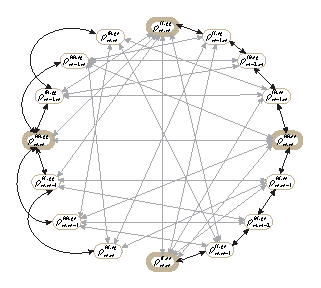
\includegraphics[width=9cm]{master.eps}
%\caption{Self-consistent hierarchy of the dynamical equations without the dipole-dipole interaction.}
%\label{figure:master-p}
%\end{figure}
%
In the steady state, $\frac{d}{dt}\rho_{m,n}^{ij,i^{\prime}j^{\prime}}=0$, we can get a coupled set of linear equations. Then the occupation probability of the cavity mode $p_{m}$ can be expressed as
\begin{equation}
\begin{split}
p_{m}=\rho_{m,m}^{hh,gg}+\rho_{m,m}^{hh,ee}+\rho_{m,m}^{ll,gg}+\rho_{m,m}^{ll,ee}.
\end{split}
\label{pm}
\end{equation}
It is worth pointing out that one must use the normalization condition when solving $p_{m}$, that is, $\sum_{m}(\rho_{m,m}^{hh,gg}+\rho_{m,m}^{hh,ee}+\rho_{m,m}^{ll,gg}+\rho_{m,m}^{ll,ee})=1$.
The whole coupling scheme of dynamical quantities in right side of Eq.~\ref{pm} fulfilling a self-consistent hierarchy of dynamical equations.
%as depicted in Fig.~\ref{figure:master-p}. 
\revision{To solve these equations, the photonic Hilbert space must be truncated at a crucial order $N$ of the photon states.  The total number of equations is $16(N+1)^{2}$. Finally, the numerical solution can be performed by using the Gauss-Jordan elimination. In our calculations, it is enough to take $N=100$.}

\begin{figure}[h]
\centering
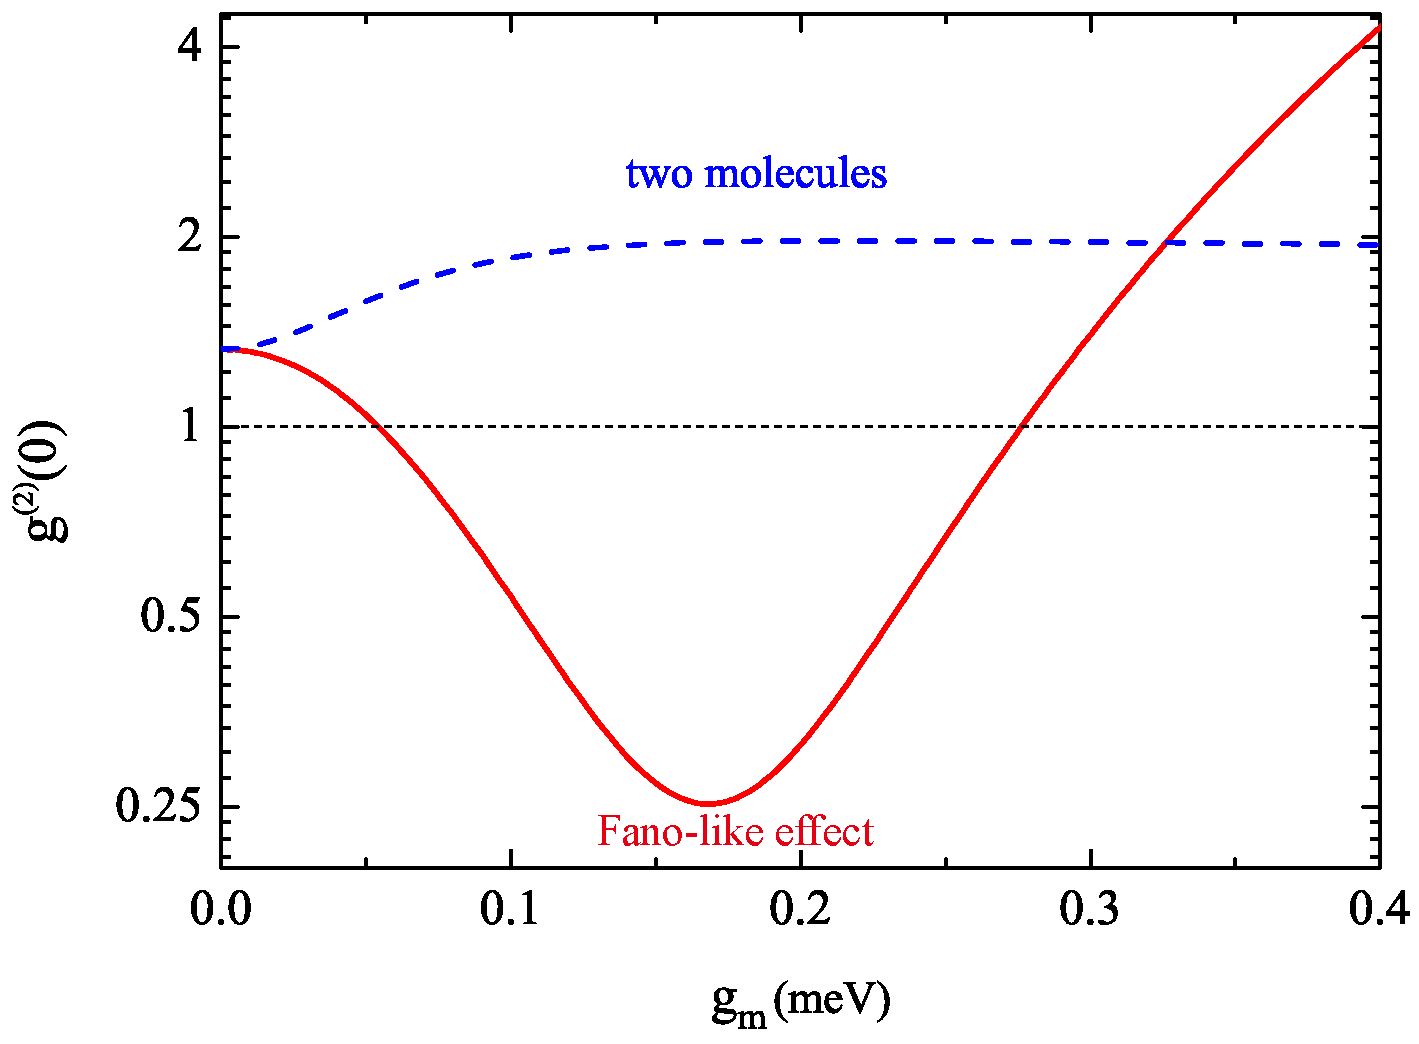
\includegraphics[width=8cm]{fano-mep.pdf}
\caption{Semilogarithmic plot of the second-order photon correlation function $g^{(2)}(0)$ as a function of the molecule-cavity coupling strength $g_{m}$ for the models (c) and (d) in Fig.~2 of main text.}
\label{fano-mep}
\end{figure}
\section{$g_{m}$-dependent photon statistics}
\label{gm-photon}
The molecule-cavity coupling strength $g_{m}$ can be adjusted by tuning the relative distance between two molecules.
 Figure \ref{fano-mep} shows $g^{(2)}(0)$ at
$E_{m}=0$ and $E_{m}=0.1~{\rm meV}$ as a function of the molecule-cavity coupling $g_{m}$ when the energy detuning vanishes, that is, $\Delta_{pm}=0$.
By increasing $g_{m}$, one notices that $g^{(2)}(0)$ displays a clear minimum at $g_{m}\approx 0.18~{\rm meV}$ that indicates the existence of Fano-like interference, see solid line in Fig.~\ref{fano-mep}.
Thus, a strong photon anti-bunching $g^{(2)}(0)\approx0.25$ can be obtained.
We see that the dip feature of $g^{(2)}(0)$ does not survive in the plot for two-molecule emission (see dashed line in Fig.~\ref{fano-mep}), which can further clarify the role of the Fano-like effect on photon statistics, as discussed in Fig.~2 of main text.


\iffalse
\section{Verification of no photon blockade}
\label{photon blockade}
According to Eq.~\ref{gn}, we can calculate the equal-time third-order photon correlation function $g^{(3)}(0)$ in Fig.~\ref{figure:g3}.
For comparison, the equal-time second-order photon correlation function $g^{(2)}(0)$ discussed in Fig.~\ref{fano-compare} is also displayed.
One can see that $g^{(3)}(0)$ shares the same trand with $g^{(2)}(0)$ but with smaller (stronger) anti-bunching (bunching) under resonance (non-resonance) mechanism,
that is, $g^{(2)}(0)<g^{(3)}(0)<1$ at $\Delta_{pm}=0$ and $g^{(3)}(0)>g^{(2)}(0)>1$ at $\Delta_{pm}\neq0$, respectively.
This violates the definition of the photon blockade\cite{PhysRevA.87.023809,PhysRevA.90.023846}. Thus, the photon anti-bunching in Fig.~\ref{fano-compare} is not caused by the photon blockade.
\begin{figure}
\centering
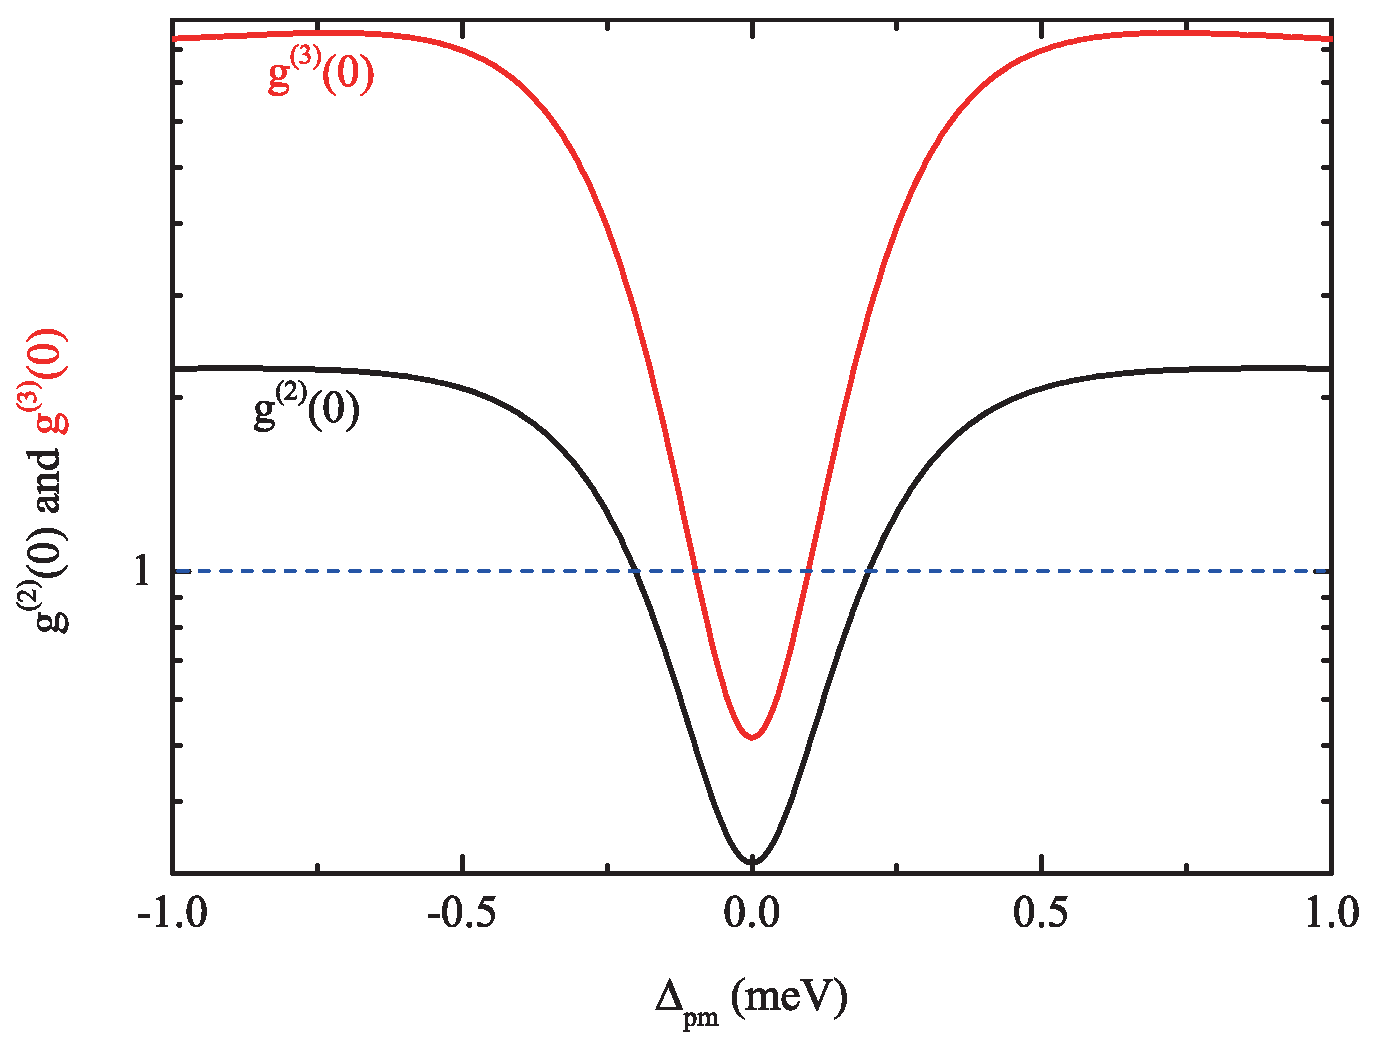
\includegraphics[width=9cm]{g3.eps}
\caption{Second- and third-order photon correlation functions $g^{(2)}(0)$ and $g^{(3)}(0)$ as a function of the energy detuning $\Delta_{pm}$.}
\label{figure:g3}
\end{figure}



\section{Simulations of photon statistics from single-molecule emission in a STM junction}
\label{STM-emission}
In this section, we simulate the single-photon emission from a single molecule driven by inelastic currents injected from a STM tip\cite{zhang2017electrically}.
In this experiment, a antibunched photon can be emitted from the decoupled single molecule from the substrate. In our model, we can set $E_{p}=0$ and $m_{ep}=0$ to simulate the single-photon emission from the single molecule as used in this experiment. The main observation of this experiment is that the photon anti-bunching becomes more and more obvious as the molecule is gradually decoupled from the substrate. We can simulate this process by studying the the evolution of second-order photon correlation function $g^{(2)}(0)$ with the inverse of the decay rate $\gamma_{dp}$ of the molecule, see Fig.~\ref{figure:STM}. Our results are in good agreement with the experiment, that is, $g^{(2)}(0)$ is decreased by
increasing $1/\gamma_{dp}$.
%
\begin{figure}
\centering
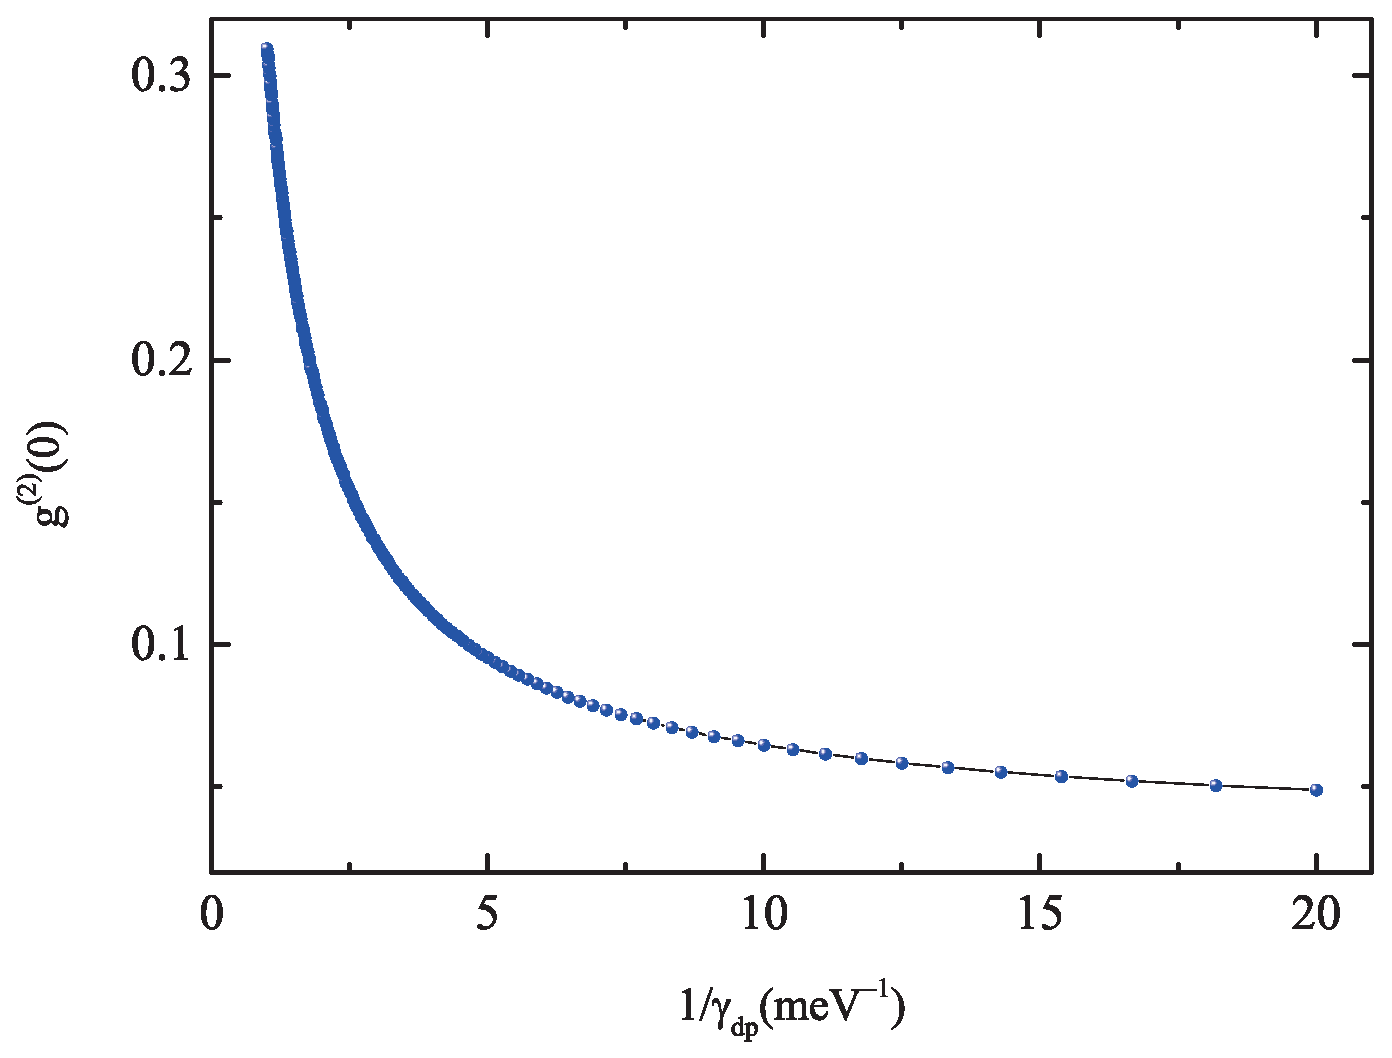
\includegraphics[width=9cm]{stm.eps}
\caption{Second-order photon correlation function $g^{(2)}(0)$ as a function of the inverse of decay rate $\gamma_{dp}$ of the molecule $p$.}
\label{figure:STM}
\end{figure}

\section{Photon density and correlation}
Figure \ref{figure:correlation1} can be used to explain the photon statistics of two-molecule emission in Fig.~\ref{fano-compare}. Figure \ref{figure:correlation} is plotted for Fig.~\ref{fano-mep}, which can clarify the non-monotonic behavior of $g^{(2)}(0)$ with $m_{ep}$.

\begin{figure}
\centering
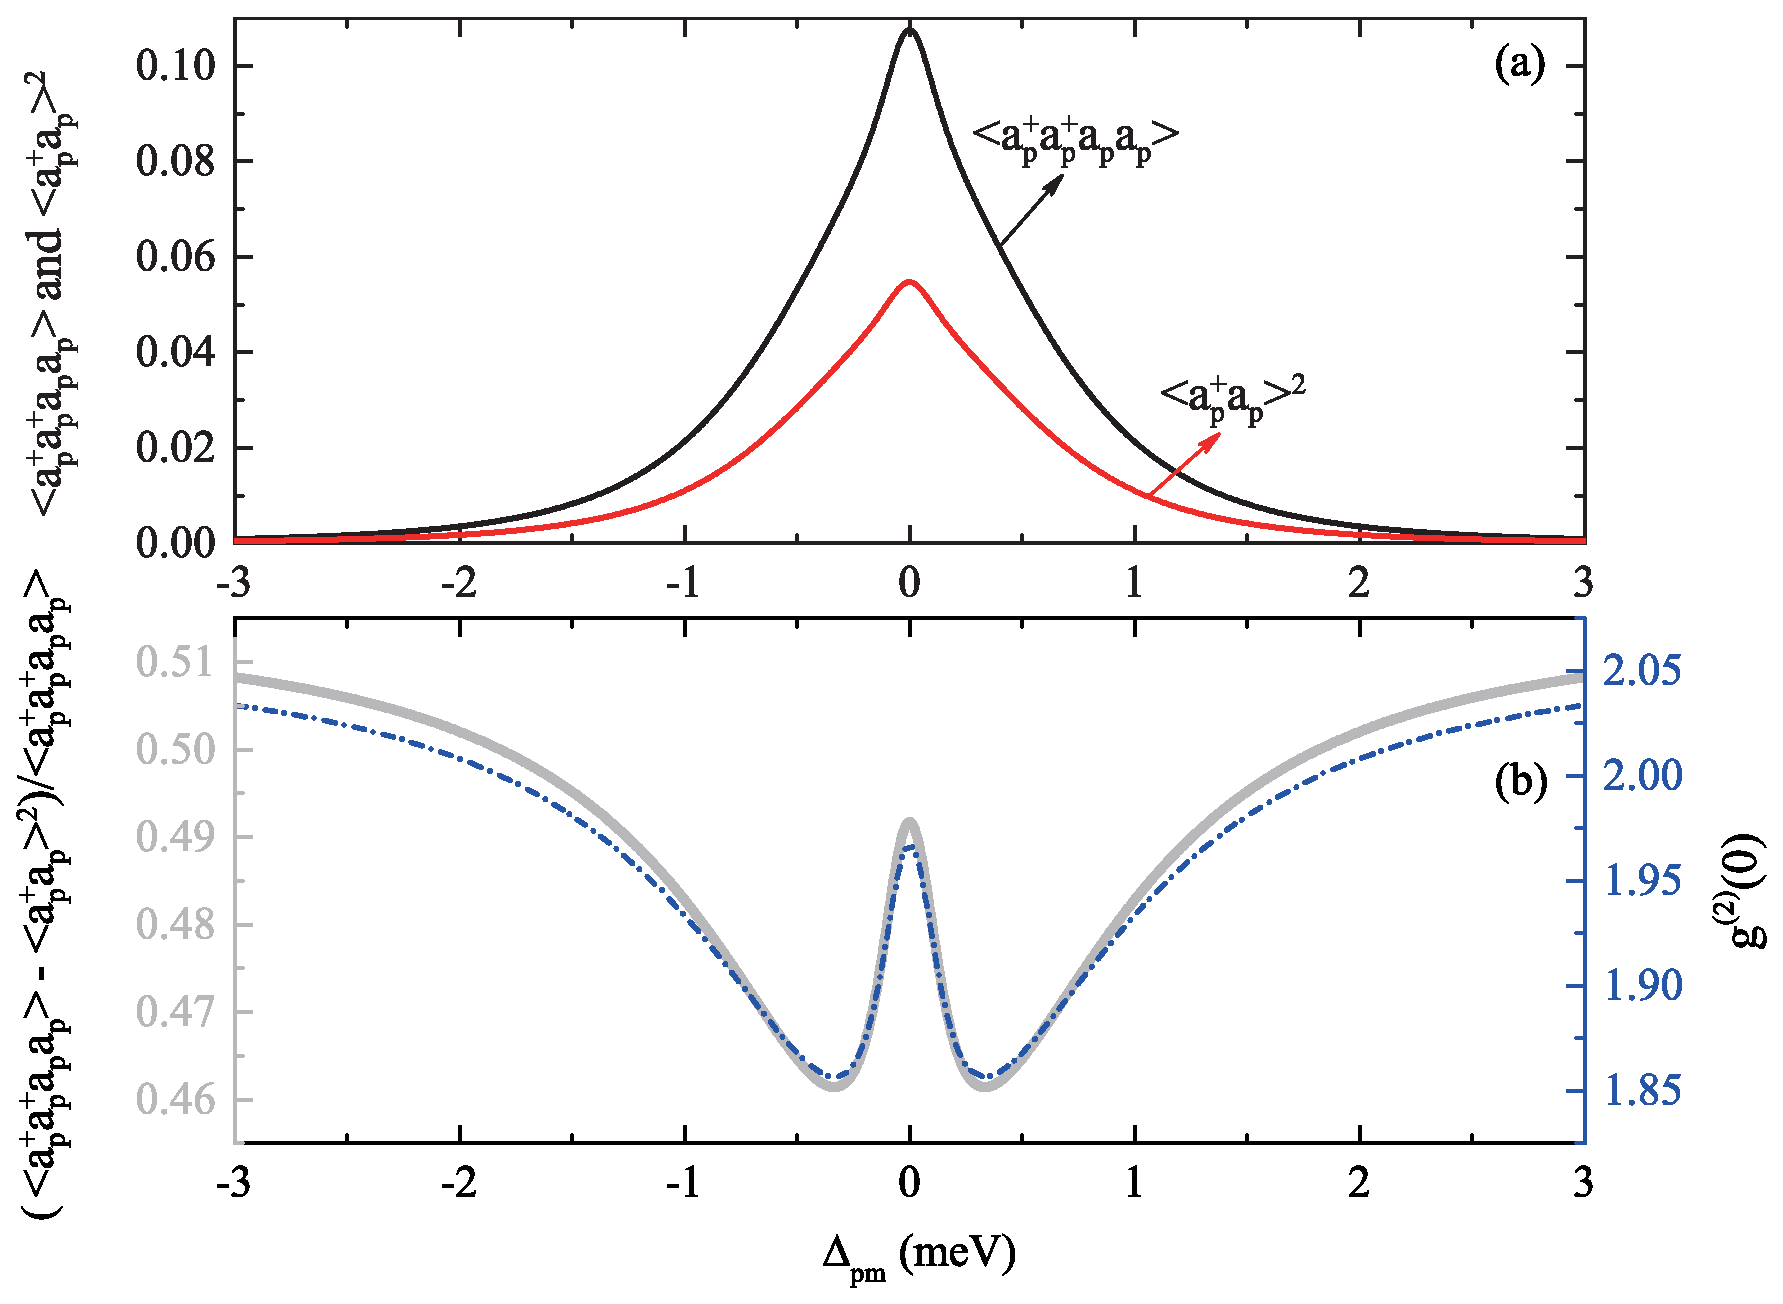
\includegraphics[width=11cm]{correlation1.eps}
\caption{(a) The photon correlation $\langle a_{p}^{\dagger}a_{p}^{\dagger}a_{p}a_{p}\rangle$ and the square of the photon density  $\langle a_{p}^{\dagger}a_{p}\rangle^{2}$ as a function of the energy detuning $\Delta_{pm}$. (b) Similar to (a) but for $\langle a_{p}^{\dagger}a_{p}^{\dagger}a_{p}a_{p}\rangle$-$\langle a_{p}^{\dagger}a_{p}\rangle^{2}$ and second-order photon correlation function $g^{(2)}(0)$.}
\label{figure:correlation1}
\end{figure}
%
\begin{figure}
\centering
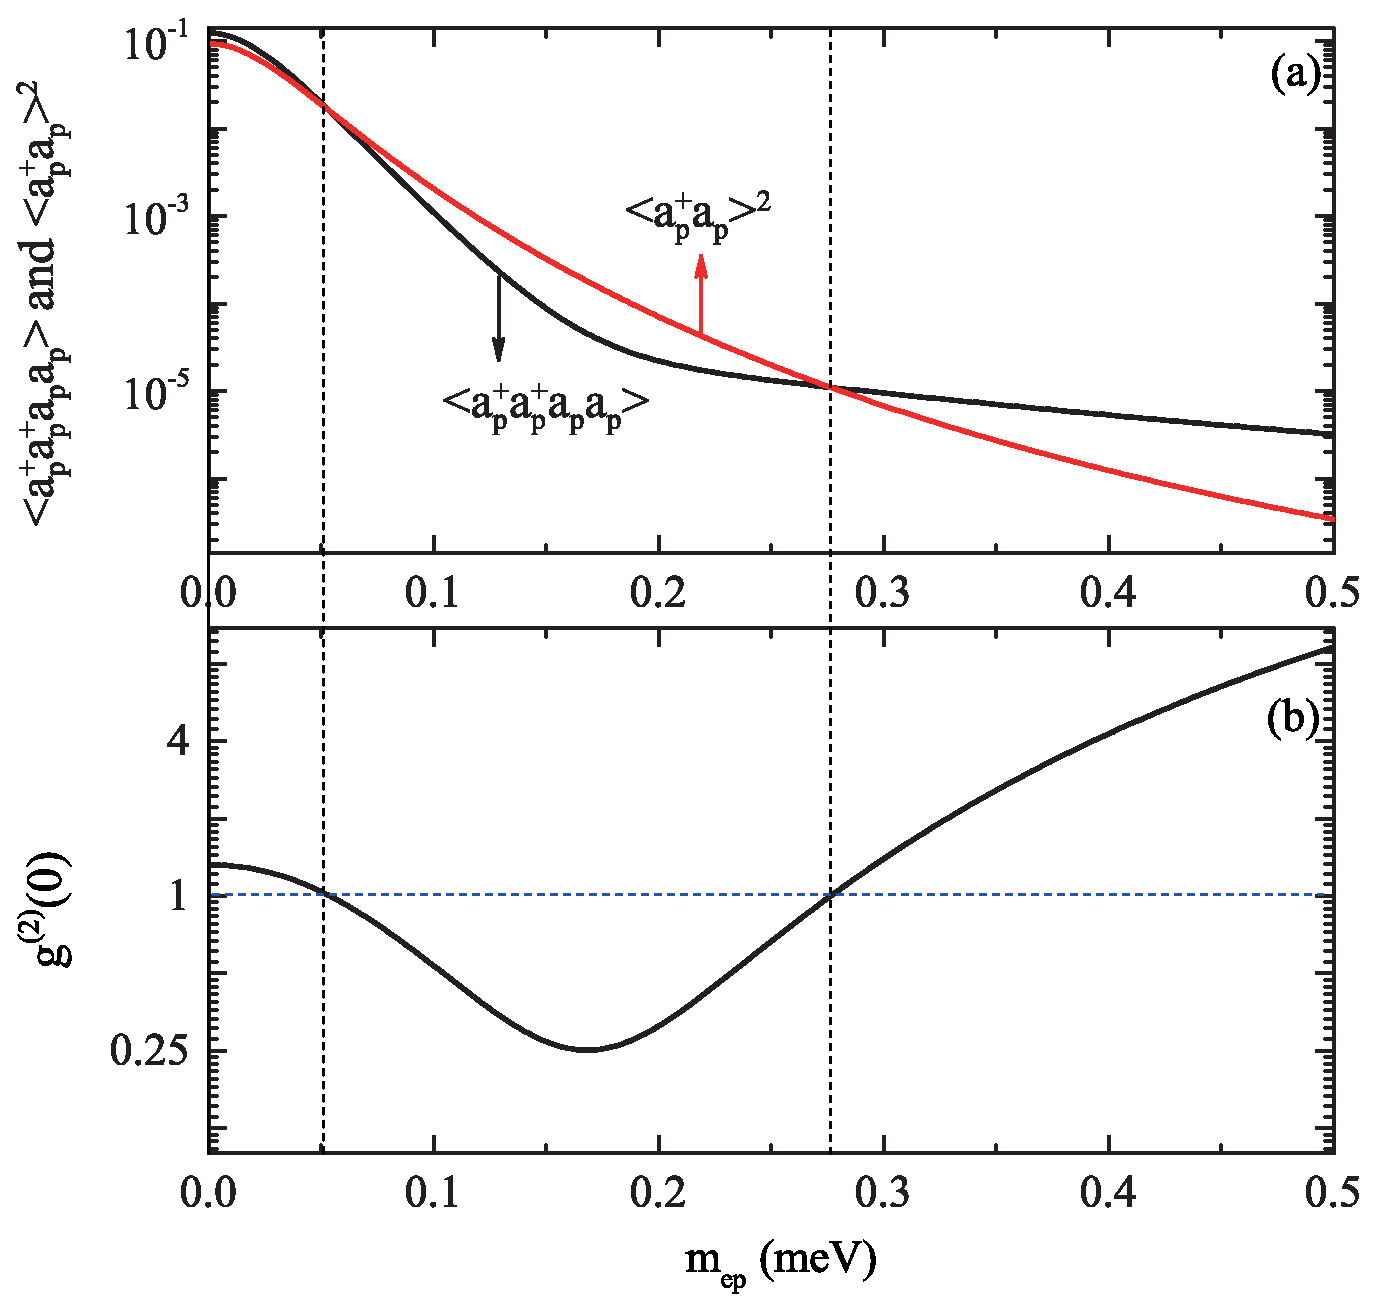
\includegraphics[width=9cm]{correlation.eps}
\caption{(a) The photon correlation $\langle a_{p}^{\dagger}a_{p}^{\dagger}a_{p}a_{p}\rangle$ and the square of the photon density  $\langle a_{p}^{\dagger}a_{p}\rangle^{2}$ as a function of the molecule-cavity coupling strength $m_{ep}$. (b) Similar to (a) but for second-order photon correlation function $g^{(2)}(0)$.}
\label{figure:correlation}
\end{figure}
\fi

\end{document}

%
% ****** End of file apstemplate.tex ******

